\section{Expansion of Maxwell's Curl Equations in Cartesian Coordinates}

The Maxwell's equations are:

\begin{eqnarray}
    \rot \Et(t) = & -\partial _t \Bt(t), \\
    \rot \Hht(t) = & \partial_t \Dt(t), \\
    \Div \Bt(t) = & 0, \\
    \Div \Dt(t) = & 0,
\end{eqnarray}
where $\partial_t\cdot = \partialDerivative{\cdot}{t}$.

The the constitutive relations are:
\begin{eqnarray}
    \Bt(t) = & \brackets{\mu_0\mu_r  (t)} \ast \Hht(t), \\
    \Dt(t) = & \brackets{\epsilon_0 \epsilon_r  (t)} \ast \Et(t),
\end{eqnarray}
where $\brackets{\cdot}$ represents a tensor.

\subsection{Normalizing the Electric Fields}
It will be adopted the conventional approach in FDTD and the electric field will be normalized as:
\begin{equation}
    \tilde{\Et}(t) = \sqrt{\cfrac{\epsilon_0}{\mu_0}}\Et(t) = \cfrac{1}{\eta_0}\Et(t).
\end{equation}
Also, from now on, the time depency $(t)$ will be ommited for cleaning notation reasons.

The other parameters related to the electric field must also be normalized:
\begin{equation}
    \tilde{\Dt} = \sqrt{\cfrac{1}{\epsilon_0\mu_0}} \Dt = c_0 \Dt.
\end{equation}

Therefore, the normalized Maxwell's equations become:

\begin{eqnarray}
    \rot \En = & -\partial _t \Bt, \\
    \rot \Hht = & \partial_t \Dn, \\
    \Div \Bt = & 0, \\
    \Div \Dn = & 0.
\end{eqnarray}


\subsection{Expanding Maxwell's Equations}

To expand the equations, it will be assumed that $\brackets{\mu_r}$ and $\brackets{\epsilon_r}$ has only diagonal terms. 

The equation $\rot \En = - \cfrac{\brackets{\mu_r}}{c_0} \partial _t \Bt$ becomes:

\begin{eqnarray}
    \partial_z\En_y - \partial_y\En_z =& \cfrac{\mu_{xx}}{c_0} \partial_t \Hht_x, \\
    \partial_x\En_z - \partial_z\En_x =& \cfrac{\mu_{yy}}{c_0} \partial_t \Hht_y,\\
    \partial_y\En_x - \partial_x\En_y =& \cfrac{\mu_{zz}}{c_0} \partial_t \Hht_z.
\end{eqnarray}

The equation $\rot \Hht = \cfrac{1}{c_0} \partial _t \Dn$ becomes:

\begin{eqnarray}
    \partial_z\Hht_y - \partial_y\Hht_z =& \cfrac{1}{c_0} \partial_t \Dn_x, \\
    \partial_x\Hht_z - \partial_z\Hht_x =& \cfrac{1}{c_0} \partial_t \Dn_y, \\
    \partial_y\Hht_x - \partial_x\Hht_y =& \cfrac{1}{c_0} \partial_t \Dn_z.
\end{eqnarray}

Finally, the equation $ \Dn = \brackets{\epsilon_r} \En $ becomes:

\begin{eqnarray}
    \Dn_x =& \epsilon_{xx} \En_x, \\
    \Dn_y =& \epsilon_{yy} \En_y, \\
    \Dn_z =& \epsilon_{zz} \En_z.
\end{eqnarray}

\subsection{Notation for Curl Terms}

\begin{eqnarray}
    \CEx =& \partial_z\En_y - \partial_y\En_z, \\
    \CEy =& \partial_x\En_z - \partial_z\En_x, \\
    \CEz =& \partial_y\En_x - \partial_x\En_y.
\end{eqnarray}

\begin{eqnarray}
    \CHx =& \partial_z\Hht_y - \partial_y\Hht_z, \\
    \CHy =& \partial_x\Hht_z - \partial_z\Hht_x, \\
    \CHz =& \partial_y\Hht_x - \partial_x\Hht_y.
\end{eqnarray}

\subsection{Final Equations Form}

\begin{eqnarray}
    \CEx =& \cfrac{\mu_{xx}}{c_0} \partial_t \Hht_x, \\
    \CEy =& \cfrac{\mu_{yy}}{c_0} \partial_t \Hht_y,\\
    \CEz =& \cfrac{\mu_{zz}}{c_0} \partial_t \Hht_z.
\end{eqnarray}

\begin{eqnarray}
    \CHx =& \cfrac{1}{c_0} \partial_t \Dn_x, \\
    \CHy =& \cfrac{1}{c_0} \partial_t \Dn_y, \\
    \CHz =& \cfrac{1}{c_0} \partial_t \Dn_z.
\end{eqnarray}

\begin{eqnarray}
    \Dn_x =& \epsilon_{xx} \En_x, \\
    \Dn_y =& \epsilon_{yy} \En_y, \\
    \Dn_z =& \epsilon_{zz} \En_z.
\end{eqnarray}


\section{Finite-Difference Approximation to Maxwell's Equations}

\subsection{Yee Grid}
A unit cell is constructed by dividing the 3 axis into discrete cells of size $(\dx, \dy, \dz)$. Inside this cell, it is necessary to put all the fields of the electromagnetic problem $(\Et_x, \Et_y, \Et_z, \Hht_x, \Hht_x, \Hht_z)$. Instead of putting all fields on the origin $(0, 0, 0)$, where is more intuitive, Yee proposed the following approach:



\tikzset{every picture/.style={line width=0.75pt}} %set default line width to 0.75pt        

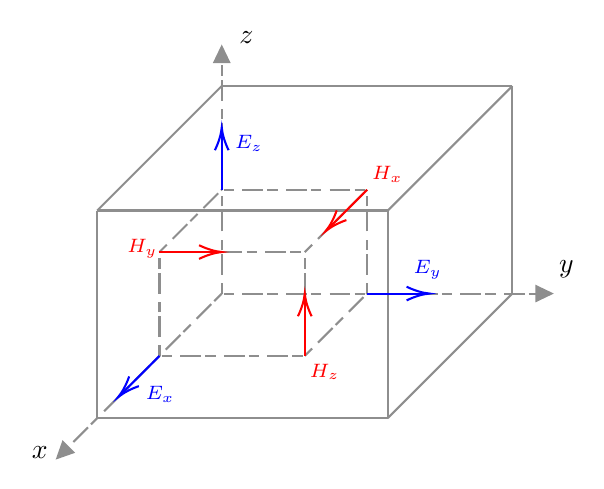
\begin{tikzpicture}[x=0.75pt,y=0.75pt,yscale=-1,xscale=1]
%uncomment if require: \path (0,300); %set diagram left start at 0, and has height of 300

%Straight Lines [id:da7206106706219195] 
\draw [color={rgb, 255:red, 142; green, 142; blue, 142 }  ,draw opacity=1 ]   (235,130) -- (235,30) ;
%Straight Lines [id:da33698179602076084] 
\draw [color={rgb, 255:red, 142; green, 142; blue, 142 }  ,draw opacity=1 ]   (35,190) -- (175,190) ;
%Straight Lines [id:da9138355462483165] 
\draw [color={rgb, 255:red, 142; green, 142; blue, 142 }  ,draw opacity=1 ]   (35,190) -- (35,90) ;
%Straight Lines [id:da685935512376388] 
\draw [color={rgb, 255:red, 142; green, 142; blue, 142 }  ,draw opacity=1 ]   (35,90) -- (175,90) ;
%Straight Lines [id:da445111134636218] 
\draw [color={rgb, 255:red, 142; green, 142; blue, 142 }  ,draw opacity=1 ]   (175,190) -- (235,130) ;
%Straight Lines [id:da484524333762936] 
\draw [color={rgb, 255:red, 142; green, 142; blue, 142 }  ,draw opacity=1 ]   (175,90) -- (235,30) ;
%Straight Lines [id:da9913295376298443] 
\draw [color={rgb, 255:red, 142; green, 142; blue, 142 }  ,draw opacity=1 ]   (35,90) -- (95,30) ;
%Straight Lines [id:da5460324336870037] 
\draw [color={rgb, 255:red, 142; green, 142; blue, 142 }  ,draw opacity=1 ]   (95,30) -- (235,30) ;
%Straight Lines [id:da6638914765185959] 
\draw [color={rgb, 255:red, 142; green, 142; blue, 142 }  ,draw opacity=1 ] [dash pattern={on 3.75pt off 3pt on 7.5pt off 1.5pt}]  (95,130) -- (95,13) ;
\draw [shift={(95,10)}, rotate = 90] [fill={rgb, 255:red, 142; green, 142; blue, 142 }  ,fill opacity=1 ][line width=0.08]  [draw opacity=0] (8.93,-4.29) -- (0,0) -- (8.93,4.29) -- cycle    ;
%Straight Lines [id:da5590643789875542] 
\draw [color={rgb, 255:red, 142; green, 142; blue, 142 }  ,draw opacity=1 ] [dash pattern={on 3.75pt off 3pt on 7.5pt off 1.5pt}]  (96,130) -- (252,130) ;
\draw [shift={(255,130)}, rotate = 180] [fill={rgb, 255:red, 142; green, 142; blue, 142 }  ,fill opacity=1 ][line width=0.08]  [draw opacity=0] (8.93,-4.29) -- (0,0) -- (8.93,4.29) -- cycle    ;
%Straight Lines [id:da13059528999125825] 
\draw [color={rgb, 255:red, 142; green, 142; blue, 142 }  ,draw opacity=1 ] [dash pattern={on 3.75pt off 3pt on 7.5pt off 1.5pt}]  (17.12,207.88) -- (95,130) ;
\draw [shift={(15,210)}, rotate = 315] [fill={rgb, 255:red, 142; green, 142; blue, 142 }  ,fill opacity=1 ][line width=0.08]  [draw opacity=0] (8.93,-4.29) -- (0,0) -- (8.93,4.29) -- cycle    ;
%Straight Lines [id:da6668538193606308] 
\draw [color={rgb, 255:red, 142; green, 142; blue, 142 }  ,draw opacity=1 ]   (175,190) -- (175,90) ;
%Straight Lines [id:da383295540871357] 
\draw [color={rgb, 255:red, 142; green, 142; blue, 142 }  ,draw opacity=1 ] [dash pattern={on 3.75pt off 3pt on 7.5pt off 1.5pt}]  (165,130) -- (165,80) ;
%Straight Lines [id:da3974993340565597] 
\draw [color={rgb, 255:red, 142; green, 142; blue, 142 }  ,draw opacity=1 ] [dash pattern={on 3.75pt off 3pt on 7.5pt off 1.5pt}]  (65,160) -- (65,110) ;
%Straight Lines [id:da44160642910672465] 
\draw [color={rgb, 255:red, 142; green, 142; blue, 142 }  ,draw opacity=1 ] [dash pattern={on 3.75pt off 3pt on 7.5pt off 1.5pt}]  (135,160) -- (135,110) ;
%Straight Lines [id:da5629234248062879] 
\draw [color={rgb, 255:red, 142; green, 142; blue, 142 }  ,draw opacity=1 ] [dash pattern={on 3.75pt off 3pt on 7.5pt off 1.5pt}]  (66,160) -- (135,160) ;
%Straight Lines [id:da5422854229817635] 
\draw [color={rgb, 255:red, 142; green, 142; blue, 142 }  ,draw opacity=1 ] [dash pattern={on 3.75pt off 3pt on 7.5pt off 1.5pt}]  (65,110) -- (135,110) ;
%Straight Lines [id:da6116059635293223] 
\draw [color={rgb, 255:red, 142; green, 142; blue, 142 }  ,draw opacity=1 ] [dash pattern={on 3.75pt off 3pt on 7.5pt off 1.5pt}]  (96,80) -- (165,80) ;
%Straight Lines [id:da9246979014557115] 
\draw [color={rgb, 255:red, 142; green, 142; blue, 142 }  ,draw opacity=1 ] [dash pattern={on 3.75pt off 3pt on 7.5pt off 1.5pt}]  (65,110) -- (95,80) ;
%Straight Lines [id:da7936751206446481] 
\draw [color={rgb, 255:red, 142; green, 142; blue, 142 }  ,draw opacity=1 ] [dash pattern={on 3.75pt off 3pt on 7.5pt off 1.5pt}]  (135,110) -- (165,80) ;
%Straight Lines [id:da5136819716767439] 
\draw [color={rgb, 255:red, 142; green, 142; blue, 142 }  ,draw opacity=1 ] [dash pattern={on 3.75pt off 3pt on 7.5pt off 1.5pt}]  (135,160) -- (165,130) ;
%Straight Lines [id:da7961144391033157] 
\draw [color={rgb, 255:red, 255; green, 0; blue, 0 }  ,draw opacity=1 ]   (65,110) -- (93,110) ;
\draw [shift={(95,110)}, rotate = 180] [color={rgb, 255:red, 255; green, 0; blue, 0 }  ,draw opacity=1 ][line width=0.75]    (10.93,-3.29) .. controls (6.95,-1.4) and (3.31,-0.3) .. (0,0) .. controls (3.31,0.3) and (6.95,1.4) .. (10.93,3.29)   ;
%Straight Lines [id:da12124972293983005] 
\draw [color={rgb, 255:red, 255; green, 0; blue, 0 }  ,draw opacity=1 ]   (165,80) -- (146.41,98.59) ;
\draw [shift={(145,100)}, rotate = 315] [color={rgb, 255:red, 255; green, 0; blue, 0 }  ,draw opacity=1 ][line width=0.75]    (10.93,-3.29) .. controls (6.95,-1.4) and (3.31,-0.3) .. (0,0) .. controls (3.31,0.3) and (6.95,1.4) .. (10.93,3.29)   ;
%Straight Lines [id:da3302622370080578] 
\draw [color={rgb, 255:red, 255; green, 0; blue, 0 }  ,draw opacity=1 ]   (135,160) -- (135,132) ;
\draw [shift={(135,130)}, rotate = 90] [color={rgb, 255:red, 255; green, 0; blue, 0 }  ,draw opacity=1 ][line width=0.75]    (10.93,-3.29) .. controls (6.95,-1.4) and (3.31,-0.3) .. (0,0) .. controls (3.31,0.3) and (6.95,1.4) .. (10.93,3.29)   ;
%Straight Lines [id:da5288808191623237] 
\draw [color={rgb, 255:red, 0; green, 0; blue, 255 }  ,draw opacity=1 ]   (95,80) -- (95,52) ;
\draw [shift={(95,50)}, rotate = 90] [color={rgb, 255:red, 0; green, 0; blue, 255 }  ,draw opacity=1 ][line width=0.75]    (10.93,-3.29) .. controls (6.95,-1.4) and (3.31,-0.3) .. (0,0) .. controls (3.31,0.3) and (6.95,1.4) .. (10.93,3.29)   ;
%Straight Lines [id:da13848590216057788] 
\draw [color={rgb, 255:red, 0; green, 0; blue, 255 }  ,draw opacity=1 ]   (65,160) -- (46.41,178.59) ;
\draw [shift={(45,180)}, rotate = 315] [color={rgb, 255:red, 0; green, 0; blue, 255 }  ,draw opacity=1 ][line width=0.75]    (10.93,-3.29) .. controls (6.95,-1.4) and (3.31,-0.3) .. (0,0) .. controls (3.31,0.3) and (6.95,1.4) .. (10.93,3.29)   ;
%Straight Lines [id:da9041413940467059] 
\draw [color={rgb, 255:red, 0; green, 0; blue, 255 }  ,draw opacity=1 ]   (165,130) -- (193,130) ;
\draw [shift={(195,130)}, rotate = 180] [color={rgb, 255:red, 0; green, 0; blue, 255 }  ,draw opacity=1 ][line width=0.75]    (10.93,-3.29) .. controls (6.95,-1.4) and (3.31,-0.3) .. (0,0) .. controls (3.31,0.3) and (6.95,1.4) .. (10.93,3.29)   ;

% Text Node
\draw (2,202.4) node [anchor=north west][inner sep=0.75pt]    {$x$};
% Text Node
\draw (256,112.4) node [anchor=north west][inner sep=0.75pt]    {$y$};
% Text Node
\draw (102,2.4) node [anchor=north west][inner sep=0.75pt]    {$z$};
% Text Node
\draw (48,102.4) node [anchor=north west][inner sep=0.75pt]  [font=\scriptsize,color={rgb, 255:red, 255; green, 0; blue, 0 }  ,opacity=1 ]  {$H_{y}$};
% Text Node
\draw (136,162.4) node [anchor=north west][inner sep=0.75pt]  [font=\scriptsize,color={rgb, 255:red, 255; green, 0; blue, 0 }  ,opacity=1 ]  {$H_{z}$};
% Text Node
\draw (166,67.4) node [anchor=north west][inner sep=0.75pt]  [font=\scriptsize,color={rgb, 255:red, 255; green, 0; blue, 0 }  ,opacity=1 ]  {$H_{x}$};
% Text Node
\draw (57,173.4) node [anchor=north west][inner sep=0.75pt]  [font=\scriptsize,color={rgb, 255:red, 0; green, 0; blue, 255 }  ,opacity=1 ]  {$E_{x}$};
% Text Node
\draw (186,112.4) node [anchor=north west][inner sep=0.75pt]  [font=\scriptsize,color={rgb, 255:red, 0; green, 0; blue, 255 }  ,opacity=1 ]  {$E_{y}$};
% Text Node
\draw (100,52.4) node [anchor=north west][inner sep=0.75pt]  [font=\scriptsize,color={rgb, 255:red, 0; green, 0; blue, 255 }  ,opacity=1 ]  {$E_{z}$};


\end{tikzpicture}


\begin{itemize}
    \item $\Et_x$ on $(\dx/2, 0, 0)$,
    \item $\Et_y$ on $(0, \dy/2, 0)$,
    \item $\Et_z$ on $(0, 0, \dz/2)$,
    \item $\Hht_x$ on $(0, \dy/2, \dz/2)$,
    \item $\Hht_y$ on $(\dx/2, 0, \dz/2)$,
    \item $\Hht_z$ on $(\dx/2, \dy/2, 0)$.
\end{itemize}

There are some reasons for using this scheme:
\begin{itemize}
    \item The divergences are naturally zero.
    \item The physical boundary conditions are naturally satisfied.
    \item It is an elegant arrangement to approximate Maxwell's curl equations.
\end{itemize}

Additionaly, there are some consequences for using this scheme:
\begin{itemize}
    \item Field components are in physically different locations.
    \item Field components may be in different materials even if they are in the same unit cell.
    \item Field components will be out of phase.
\end{itemize}

\subsection{Finite-Difference Equations on Yee Grid}

Each cell on the grid is identified by the coordines $(i\dx, j\dy, k\dz)$, where $(i, j, k)$ are the index of the cell.

Note that on each face of the Yee cell there is the fields of the adjacent cell.

Consider, first, the grid for $\Hht_x$:

\input{contents/tiks/yee_grid_chx.tex}

Based on this schematic, it is possible to write:

\begin{eqnarray}
    \partialDerivative{\En_z^{i,j,k}}{y}(t) =& \cfrac{\En_z^{i, j+1, k}(t)-\En_z^{i, j, k}(t)}{\dy}, \\
    \partialDerivative{\En_y^{i,j,k}}{z}(t) =& \cfrac{\En_y^{i, j, k+1}(t)-\En_y^{i, j, k}(t)}{\dy}.
\end{eqnarray}

Note that this space derivatives exists at time instant $t$ and they exist at the same point as $\Hht_x^{i,j,k}$.

We need to explicitly write the time on the Yee grid equations, since it is essencial to write all the members of equations on the same time instant.

Hence, the $\CEx$ final equation is:

\begin{eqnarray}
    \CEx =& \cfrac{\En_z^{i, j+1, k}(t)-\En_z^{i, j, k}(t)}{\dy} - \nonumber \\ 
    \qquad & \cfrac{\En_y^{i, j, k+1}(t)-\En_y^{i, j, k}(t)}{\dz}
    \label{eq:CEx}
\end{eqnarray}

Now, for the time derivative $\partial_t \Hht_x$ to exists at time $t$:

\begin{equation}
    \partial_t \Hht_x^{i,j,k}(t) = \cfrac{\Hht_x^{i,j,k}(t+\nicefrac{\dt}{2}) - \Hht_x^{i,j,k}(t-\nicefrac{\dt}{2})}{\dt}.
\end{equation}

So, the finite-difference equation for $\Hht_x$ becomes:

\begin{eqnarray}
    \cfrac{\En_z^{i, j+1, k}(t)-\En_z^{i, j, k}(t)}{\dy} - \cfrac{\En_y^{i, j, k+1}(t)-\En_y^{i, j, k}(t)}{\dy} \nonumber \\ 
    =\cfrac{\mu_{xx}^{i,j,k}}{c_0}\cfrac{\Hht_x^{i,j,k}(t+\nicefrac{\dt}{2}) - \Hht_x^{i,j,k}(t-\nicefrac{\dt}{2})}{\dt}.
    \label{eq:fd_hx}
\end{eqnarray}

Similarly, it is possible to write the curl equations for the other components of $\En$ and for $\Hht$:

\begin{eqnarray}
    \CEy =& \cfrac{\En_x^{i, j, k+1}(t)-\En_x^{i, j, k}(t)}{\dz} - \nonumber \\ 
    \qquad & \cfrac{\En_z^{i+1, j, k}(t)-\En_z^{i, j, k}(t)}{\dx}
    \label{eq:CEy}
\end{eqnarray}

\begin{eqnarray}
    \CEz =& \cfrac{\En_y^{i+1, j, k}(t)-\En_y^{i, j, k}(t)}{\dx} - \nonumber \\ 
    \qquad & \cfrac{\En_x^{i, j+1, k}(t)-\En_x^{i, j+1, k}(t)}{\dy}
    \label{eq:CEz}
\end{eqnarray}

\begin{eqnarray}
    \CHx =& \cfrac{\Hht_z^{i, j, k}(t+\nicefrac{\dt}{2})-\Hht_z^{i, j-1, k}(t+\nicefrac{\dt}{2})}{\dy} - \nonumber \\ 
    \qquad & \cfrac{\Hht_y^{i, j, k}(t+\nicefrac{\dt}{2})-\Hht_y^{i, j, k-1}(t+\nicefrac{\dt}{2})}{\dz}
    \label{eq:CHx}
\end{eqnarray}


\begin{eqnarray}
    \CHy =& \cfrac{\Hht_x^{i, j, k}(t+\nicefrac{\dt}{2})-\Hht_x^{i, j, k-1}(t+\nicefrac{\dt}{2})}{\dz} - \nonumber \\ 
    \qquad & \cfrac{\Hht_z^{i, j, k}(t+\nicefrac{\dt}{2})-\Hht_z^{i-1, j, k}(t+\nicefrac{\dt}{2})}{\dx}
    \label{eq:CHy}
\end{eqnarray}


\begin{eqnarray}
    \CHz =& \cfrac{\Hht_y^{i, j, k}(t+\nicefrac{\dt}{2})-\Hht_y^{i-1, j, k}(t+\nicefrac{\dt}{2})}{\dx} - \nonumber \\ 
    \qquad & \cfrac{\Hht_x^{i, j, k}(t+\nicefrac{\dt}{2})-\Hht_x^{i, j-1, k}(t+\nicefrac{\dt}{2})}{\dy}
    \label{eq:CHz}
\end{eqnarray}

Finally, the finite-difference equations are, for $\Hht_y$:

\begin{eqnarray}
    \cfrac{\En_x^{i, j, k+1}(t)-\En_x^{i, j, k}(t)}{\dz} - \cfrac{\En_z^{i+1, j, k}(t)-\En_z^{i, j, k}(t)}{\dx} \nonumber \\ 
    =\cfrac{\mu_{yy}^{i,j,k}}{c_0}\cfrac{\Hht_y^{i,j,k}(t+\nicefrac{\dt}{2}) - \Hht_y^{i,j,k}(t-\nicefrac{\dt}{2})}{\dt},
    \label{eq:fd_hy}
\end{eqnarray}

for $\Hht_z$:

\begin{eqnarray}
    \cfrac{\En_y^{i+1, j, k}(t)-\En_y^{i, j, k}(t)}{\dx} - \cfrac{\En_x^{i, j+1, k}(t)-\En_x^{i, j+1, k}(t)}{\dy} \nonumber \\
    =\cfrac{\mu_{zz}^{i,j,k}}{c_0}\cfrac{\Hht_z^{i,j,k}(t+\nicefrac{\dt}{2}) - \Hht_z^{i,j,k}(t-\nicefrac{\dt}{2})}{\dt},
    \label{eq:fd_hz}
\end{eqnarray}

for $\En_x$:

\begin{eqnarray}
    &\cfrac{\Hht_z^{i, j, k}(t+\nicefrac{\dt}{2})-\Hht_z^{i, j-1, k}(t+\nicefrac{\dt}{2})}{\dy} - \nonumber\\ 
    & \cfrac{\Hht_y^{i, j, k}(t+\nicefrac{\dt}{2})-\Hht_y^{i, j, k-1}(t+\nicefrac{\dt}{2})}{\dz} = \nonumber\\
    &\cfrac{\epsilon_{xx}^{i,j,k}}{c_0}\cfrac{\En_x^{i,j,k}(t+\nicefrac{\dt}{2})-\En_x^{i,j,k}(t)}{\dt},
    \label{eq:fd_ex}
\end{eqnarray}

for $\En_y$:

\begin{eqnarray}
    &\cfrac{\Hht_x^{i, j, k}(t+\nicefrac{\dt}{2})-\Hht_x^{i, j, k-1}(t+\nicefrac{\dt}{2})}{\dz} - \nonumber \\
    &\cfrac{\Hht_z^{i, j, k}(t+\nicefrac{\dt}{2})-\Hht_z^{i-1, j, k}(t+\nicefrac{\dt}{2})}{\dx} = \nonumber\\
    &\cfrac{\epsilon_{yy}^{i,j,k}}{c_0}\cfrac{\En_y^{i,j,k}(t+\nicefrac{\dt}{2})-\En_y^{i,j,k}(t)}{\dt},
    \label{eq:fd_ey}
\end{eqnarray}

and for $\En_z$:

\begin{eqnarray}
    &\cfrac{\Hht_y^{i, j, k}(t+\nicefrac{\dt}{2})-\Hht_y^{i-1, j, k}(t+\nicefrac{\dt}{2})}{\dx} - \nonumber \\ 
    & \cfrac{\Hht_x^{i, j, k}(t+\nicefrac{\dt}{2})-\Hht_x^{i, j-1, k}(t+\nicefrac{\dt}{2})}{\dy} = \nonumber\\
    &\cfrac{\epsilon_{zz}^{i,j,k}}{c_0}\cfrac{\En_z^{i,j,k}(t+\nicefrac{\dt}{2})-\En_z^{i,j,k}(t)}{\dt}.
    \label{eq:fd_ez}
\end{eqnarray}


To ease the implementation, the vector $\En$ will exists at integer step times $(0, \dt, 2\dt, \dots)$ meanwhile the vector $\Hht$ will exists at half time steps $(\nicefrac{\dt}{2}, 3\nicefrac{\dt}{2}, 5\nicefrac{\dt}{2}, \dots)$.